\chapter{Fabrication}
\label{chapter:fabrication}

\section{Overview}


\section{Casting Silicone}

One of the goals of this project was to create an accessible fabrication method to reduce the complexity of creating a single robot. To create a robot with a circular shape along the length and a uniform semi-circular cross-section, we needed a way to cast the silicone around an arch-shaped inner piece, which we would remove to form the hollow chamber. We decided on the open angle of about 35$^\circ$, which determined the total length of the actuator based on the restrictions from the casting process of silicone. If the actuator were to be longer and extend further underneath itself, casting with an arch-shaped mold would not have been possible. 

The silicones chosen for this project were a platinum cure, two-part silicones from Smooth-On. We used five different silicones with Shore A Hardness ranging from 20--50: DragonSkin 20~(DS20), DragonSkin 30~(DS30), SmoothSil 940~(SS40), SmoothSil 945~(SS45), and SmoothSil 950~(SS50). The shore hardness of the actuator is related to the bending resistance: the stiffer the material, the more stress is required to achieve a particular strain. These silicones are well mixed and degassed before being poured into any molds. It is essential that any materials used during the mixing process are compatible with the silicones and will not impact the curing process. We used popsicle sticks and metal spatulas for mixing within plastic cups. Fig. \ref{fig:castingstation} contains an image of the casting station covered in paper, as any drips of each silicone part not mixed properly will never cure and can become quite sticky. 

\begin{figure}[ht]
    \centering
    \includegraphics[width=4 in]{images4/castingstation.jpeg}
    \caption{Photo of the casting station featuring Dragon Skin 20 Silicone, the scale and plastic cup for weighting each part of the 2 part silicone.}
    \label{fig:castingstation}
\end{figure}

Once we thoroughly mixed the two silicone parts, we degassed in a vacuum chamber for about 2-3 minutes or until all the large air bubbles evacuated. The mixed silicone has a viscosity similar to honey. It is easy to pour but sticks to everything. It's important to remove any air from the silicone, as if the silicone cures around the air bubbles, the little pockets ruin the uniform cross-section required for consistent bending behavior. 

\clearpage
\section{Arch-Shaped Molds}
When trying to cast this shaped actuator out of a single pour of silicone, the arch shape allows us to pour in silicone from the top, and with the help of gravity, the silicone flows down to each end of the actuator. 

With guidance from Cooper's AACE Lab staff, Harrison Tyler and Judy Li, we had access to multiple different filaments and materials to create the pieces required for casting. The first check with any mold piece not made from PLA is to ensure that the material does not inhibit the silicone's curing process. Materials with high sulfur content, for example, inhibit the curing process. 

We chose to 3D-print the outer molds with PLA filament. The mold has an arch shape so that the actuator can be cast vertically through a large pour hole, and any air would be able to escape from the top of the mold. The insert would slot into the mold in the center, creating an even semi-circular cross-section. The top of the mold had a large pour hole, and the walls maintained the height of the actuator so that we could remove any material attached to the flat side of the actuator after the silicone finished curing. 

One side of the mold had protruding sections such that the other side would fit into it; the molds fit together like puzzle pieces to maintain the constant cross-section. Fig. \ref{fig:firstmold} contains the first mold designed for casting the circular actuator, highlighting the large pour hole at the top, the slot for the insert to lock into, and the asymmetries at the bottom of the molds so that they fit together and no silicone was allowed to escape from the bottom. 

\begin{figure}[ht]
    \centering
    \includegraphics[width=6.5 in]{images4/firstmolddesign.jpg}
    \caption{Design for the first mold, left is an isometric view of the 3 pieces, right is a front view of the insert inside one side of the mold.}
    \label{fig:firstmold}
\end{figure}

\clearpage
\section{Iterations on Inserts}
\subsection{Dissolvable Inserts}
Commonly used as support material for PLA 3D prints, PVA (Polyvinyl Alcohol) is a material that is soluble in water. Fig. \ref{fig:pvainsert} contains photos of actuators fabricated using a PVA insert. After confirming that the silicone could cure around this material, we printed the first inserts out of PVA using an Ultimaker 3D printer. Since this material is rigid, only 5-10\% infill was required. The higher the infill on the insert, the more time-consuming it would be to remove it. For the support material, we used PLA filament. These single-use inserts were removed from the silicone using a hot water bath. Even though there were no problems removing the insert from the silicone post-cure, printing a new insert for every actuator used a lot of material and was time-consuming. We could use the PLA molds to cast dozens of actuators, but a single-use insert did not align with the goal of simple mass production. To confirm that the insert was removable for one of the harder silicones, we cast an SS45 actuator using a PVA insert.  

\begin{figure}[ht]
    \centering
    \includegraphics[width=5 in]{images4/pvainsert.jpg}
    \caption{Fabrication of PVA inserts: A. PVA insert printed with PLA support material. B. DS20 actuators after removing from mold. C. DS20 and SS45 actuators after removing excess silicone. D. Hollow actuators post hot water bath.}
    \label{fig:pvainsert}
\end{figure}

\clearpage
\subsection{Flexible Inserts}
At AACE Lab, we had access to a TPU (thermoplastic polyurethane) filament, similar to rubber; it is flexible and removable after the silicone cures. Based on the infill \% chosen, the TPU insert's stiffness could be tuned. The inserts were printed on the bed horizontally with no support material. The overhang created an inconsistent cross-section, so we began printing with TPU as support material. The drawback of TPU inserts was that even though they could be used to cast multiple actuators, they would begin to lose their shape over time. To combat the flexibility of the TPU insert, we used pins to hold the insert in place within the mold. Using three sets of pins, we could ensure the TPU insert would remain in the center of the mold so that the cross-section of the silicone would be uniform. We used a FormLabs Resin Printer to fabricate the pins. Once again confirming that the silicone could cure around the chosen resin, we began casting actuators using the TPU inserts. Fig. \ref{fig:tpuinsert} contains photographs of the fabrication process for the first inserts. 

\begin{figure}[ht]
    \centering
    \includegraphics[width=6.5 in]{images4/tpuinsertfab.jpg}
    \caption{Fabrication of TPU inserts: A. Molds printed from PLA. B. Solid TPU inserts printed without support material. C. Comparison of different temperature settings on print quality of TPU. D. Resin printed pins of 2 materials. E. TPU insert with holes for the pins and the removed support material. F. TPU insert with pins inside of one half of the mold.}
    \label{fig:tpuinsert}
\end{figure}

The pins created a new problem of needing to patch the holes left behind in the silicone. After casting the actuator with the TPU insert and Pins, a solid TPU insert was reinserted into the hollow silicone so we could patch the holes with more DS20 silicone. Mixing and casting more silicone to patch the holes was not ideal, but it allowed us to seal the holes and create an airtight actuator. 

\clearpage
\subsubsection{Casting with flexible insert}
Using the TPU insert with the pins to maintain the cross-section along the actuator's length, we successfully fabricated a few actuators. Photos of the fabrication process are in Fig \ref{fig:tpupinfab}. The pour hole for the mold was not large enough for all of the air bubbles to escape the top of the mold, so we cut away a small section in the center of the mold. We used 40~g of part A and 40~g of part B of the DS20 silicone to fill the mold. To hold the molds together, we used several clamps to minimize the flashing and ensure a uniform cross-section. We poured the silicone a small amount at a time, ensuring all air bubbles could rise to the top. When pouring silicone, if the silicone ribbon gets too thin, more air is introduced as it folds onto itself. Frequent tapping of the mold on the lab bench was required to ensure that all of the air escaped. 

\begin{figure}[ht]
    \centering
    \includegraphics[width=6.5 in]{images4/tpupincasting.jpg}
    \caption{Fabrication of the hollow actuator using a TPU insert and pins. A. The pins placed in the insert. B. The clamps placed on the mold with the insert inside. C. Post silicone cure. D. Removing excess silicone. E. Removing the pins and insert. F. Silicone with solid insert. G. Post patching the holes from the pins. H. Completed hollow actuator body.}
    \label{fig:tpupinfab}
\end{figure}

After the silicone cured, we used a sharp blade to cut away any flashing, the silicone at the bottom of each end, and the silicone that remained in the pour hole. After removing the pins and the TPU insert, using a small amount of IPA (isopropyl alcohol) as a lubricant, we inserted the solid TPU so the holes left behind could be patched. After cleaning up the ends to make them flat, the hollow actuator is ready for the next steps of the fabrication process, sealing both ends and adding the interface for the pressurization equipment. 

\clearpage
\subsubsection{Case Study: SS45 Silicone}
The TPU insert with pins method successfully created an airtight actuator for the soft DS20 silicone. To test if the fabrication procedure would work for stiffer silicones, we cast an actuator out of SS45 silicone. This silicone has a viscosity closer to peanut butter than honey and was laborious to mix and pour. Despite tapping the mold on the lab bench to remove the trapped air bubbles, large bubbles at the top of the mold remained. A more significant issue was that we could not remove the TPU insert. The silicone was too stiff for the end caps of the insert to slide through. We had to cut the silicone to remove the insert. Upon further inspection, a few air pockets remained inside of the silicone. Fig. \ref{fig:ss45mess} contains photos of testing the TPU insert and pins fabrication method for SS45 silicone. 

\begin{figure}[ht]
    \centering
    \includegraphics[width=6.5 in]{images4/ss45mess.jpg}
    \caption{Images of failed SS45 actuator casting attempts. A. Overflow of mold during degassing. B. Samples of gaps created by air bubbles stuck in the mold. C. Un-patchable hole left from pin. D. Swiss-cheese actuator from over degassing}
    \label{fig:ss45mess}
\end{figure}

We attempted to degas the entire mold after casting the actuator to combat the air holes that remained in the silicone. The small air pockets expanded and left the actuator with a consistency of Swiss cheese. Additionally, the pins left large holes, and since the solid TPU insert could not be slid in to patch the holes, we had to look into alternate methods of restricting the flexible insert. 

\clearpage
\subsubsection{Case Study: DS20 Spacers}
For DS20 silicone, patching the holes left behind by the pins created an airtight seal. To remove the need to patch the holes, we attempted casting actuators using rings of DS20 silicone to hold the TPU insert in place. We printed a mold to cast small semi-circular rings of DS20 silicone, then cut a piece away so that the silicone would flow past the spacers and reach the ends while casting the actuator's body. The placement of the spacers was somewhat arbitrary as we were still determining if this method would create an airtight seal. After casting the actuator and removing it from the molds, simply pulling on it would break the seal between the silicone pieces. Fig. \ref{fig:ds20spacer} contains images of this attempt centering the TPU insert inside the mold. 

\begin{figure}[ht]
    \centering
    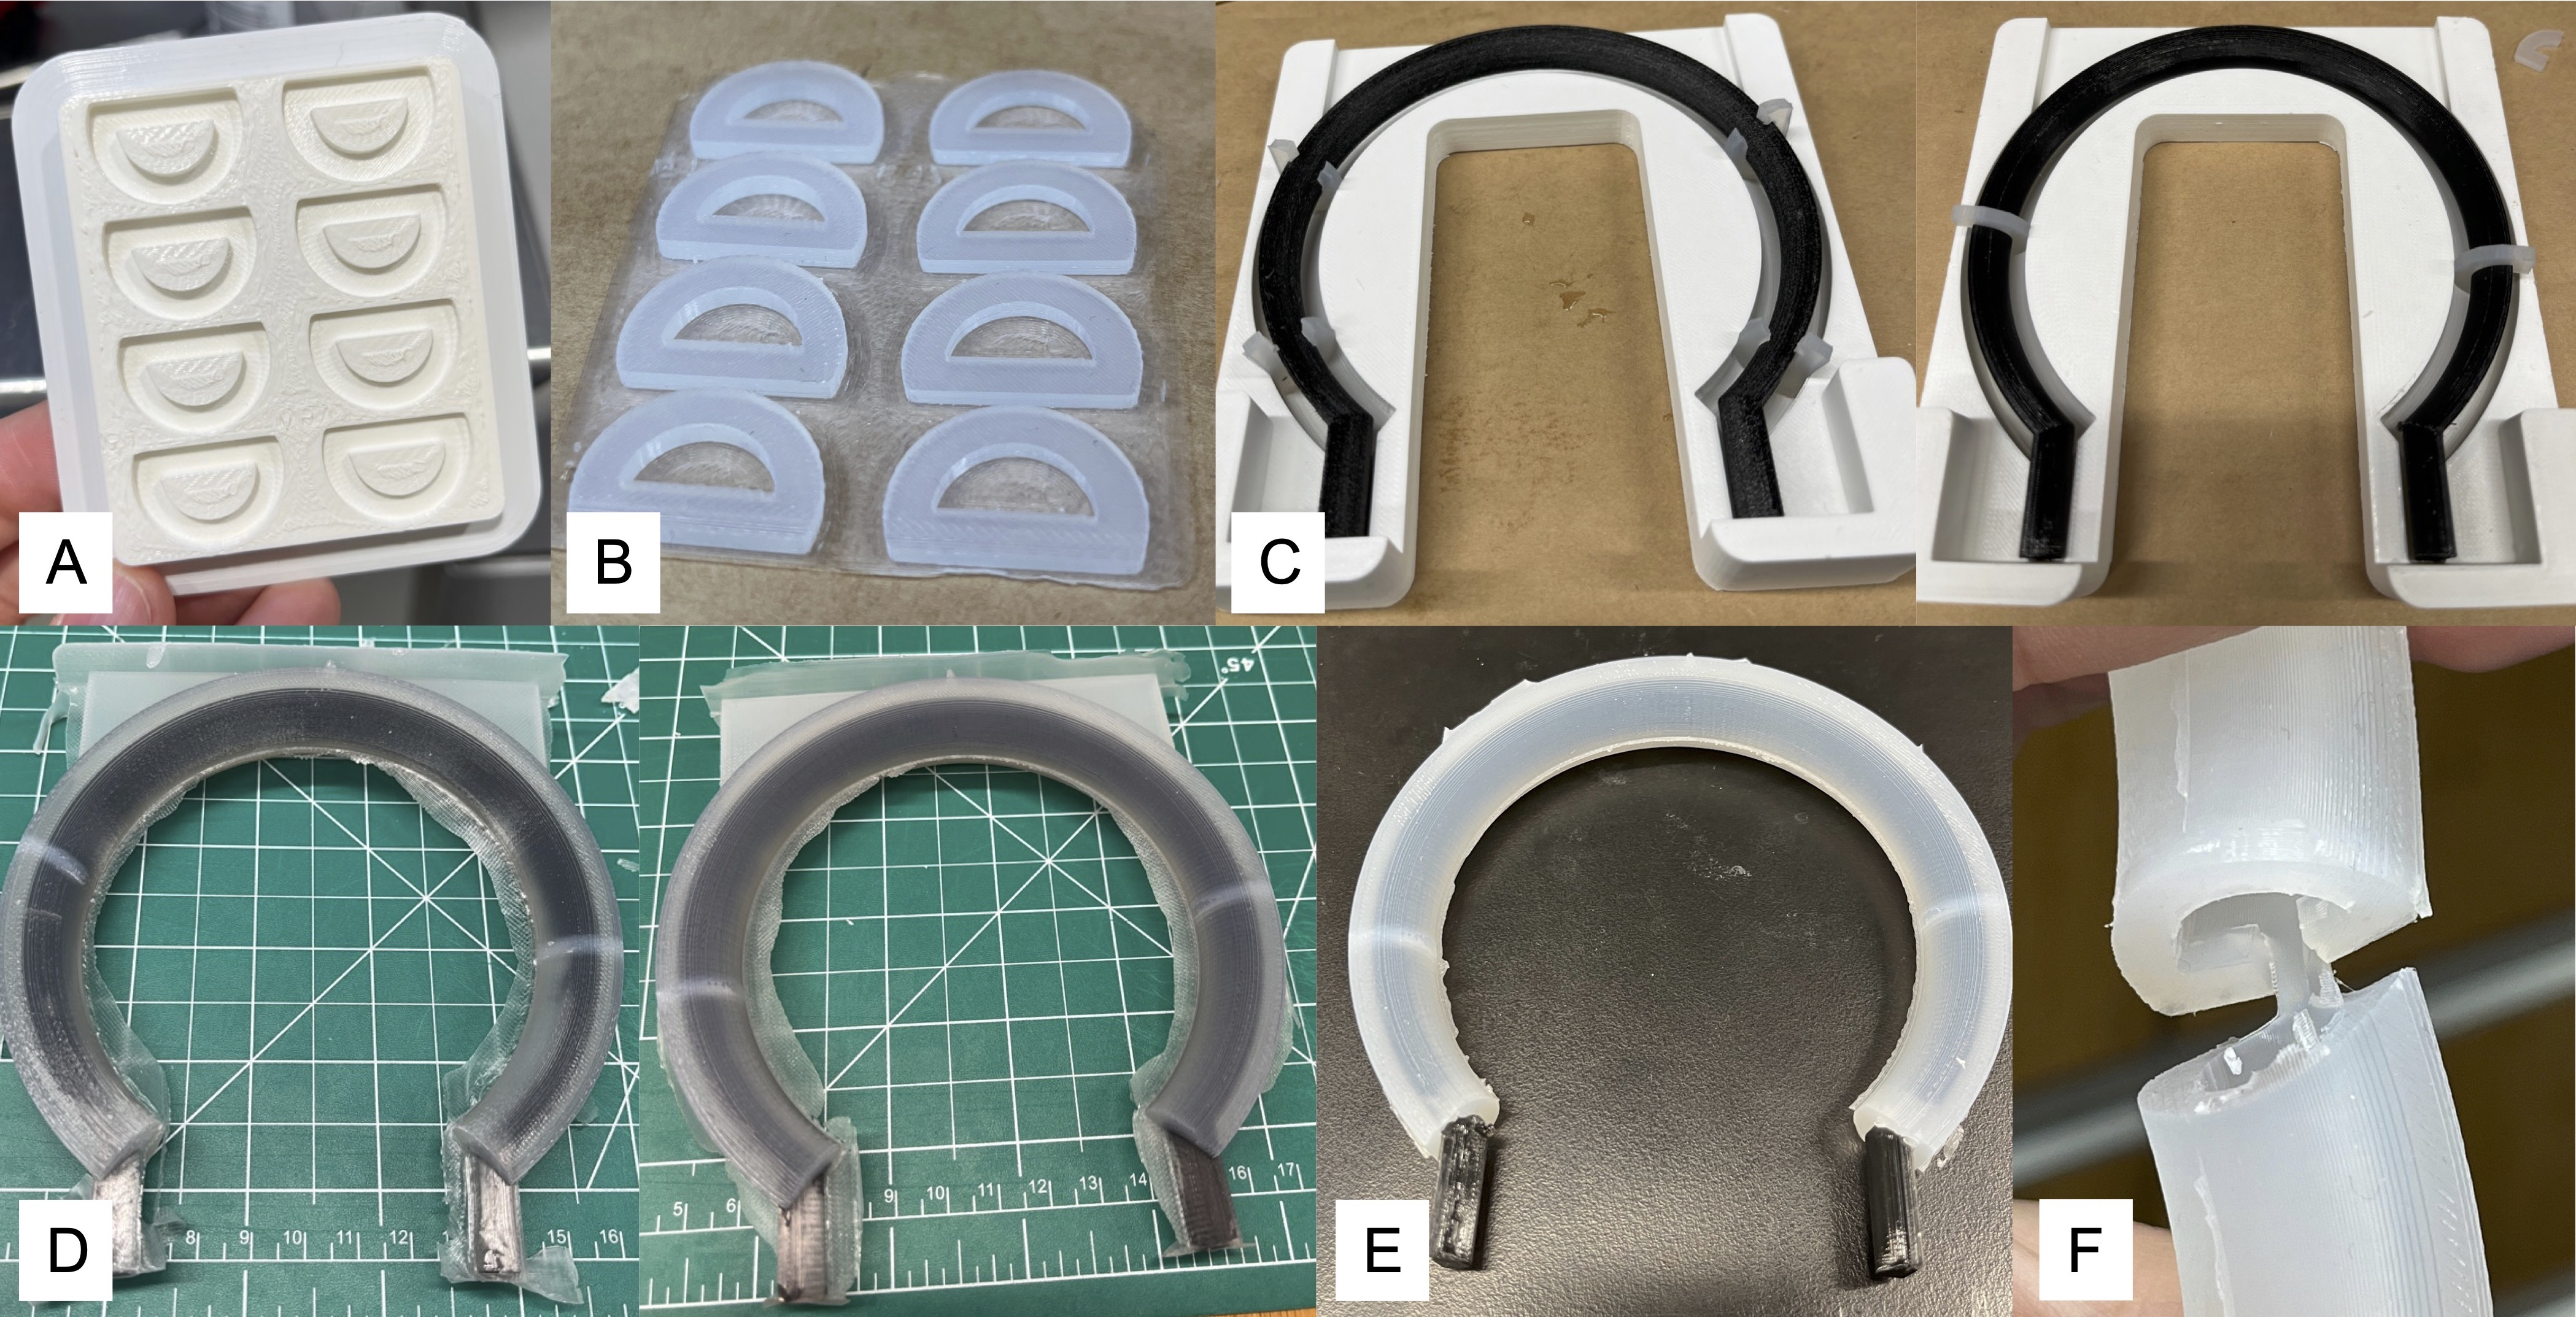
\includegraphics[width=5 in]{images4/ds20spacer.jpg}
    \caption{Images of failed attempts at using a spacer made from DS20 silicone to center the TPU insert. A. 3D printed mold for the spacers. B. casted spacers. C. Arbitrary placement of spacers. D. Casted actuators right after removing from the mold. E. After removing excess silicone. F. Failed attempt at creating a seal.}
    \label{fig:ds20spacer}
\end{figure}

\clearpage
\subsection{Wax Inserts}
Creating an insert from wax was more trouble than it was worth, but it led us closer to the final fabrication method. We found three waxes compatible with curing silicone: Beeswax, paraffin wax, and microcrystalline wax. To cast the wax insert, we 3D printed a new mold and an insert out of PLA to cast a mold from silicone. We then cast the wax into the silicone mold. 

All three waxes could be partially cast and removed from the silicone mold. However, we found that creating the wax insert to have the perfect cross-section shape to ensure a future uniform cross-section for the actuator was difficult, and the waxes were not rigid enough to hold their shape inside the mold during casting. We considered combining waxes in different ratios to enhance the stiffness and ease of casting. However, even if the wax inserts could create the perfect cross-section when casting silicone, they must be melted and recast to fabricate each actuator. With mass production in mind, we decided not to pursue wax inserts. Fig. \ref{fig:waxinserts} contains images from experimenting with wax inserts. 

\begin{figure}[ht]
    \centering
    \includegraphics[width=6 in]{images4/waxinserts.jpg}
    \caption{Experimentation with wax inserts. A. 3D printed mold and insert for casting silicone mold for wax. B. Using popsicle sticks to hold insert above silicone while casting mold. C. Paraffin wax casted in silicone mold. D. Paraffin insert removed from mold. E. Beeswax and Microcrystalline wax cast in silicone molds. F. Beeswax and Microcrystalline wax removed from silicone molds}
    \label{fig:waxinserts}
\end{figure}

\clearpage
\subsection{PCL Inserts}
PCL (polycaprolactone) is a plastic with a low melting temperature and is moldable in warm water. Using the same silicone mold made for the wax inserts, we used warm water to melt the PCL pellets into blobs, which we pressed into the silicone mold. The DS20 mold was far too flexible to shape the PCL accurately. Also, as the pieces of PCL cooled and solidified, they would not fully bond with the other pieces, leaving air gaps in the insert. After tuning the timing between the cooling down and adding more PCL pieces, we successfully created an insert and cast a DS20 actuator around the PCL insert. Unfortunately, the silicone walls were uneven, and the PCL insert had the same single-use problem as the wax inserts. Fig. \ref{fig:pclinsert} contains photographs of experimenting with PCL as an insert and the DS20 actuator we cast using the PCL insert.

\begin{figure}[ht]
    \centering
    \includegraphics[width=6 in]{images4/pclinsert.jpg}
    \caption{Experimentation with PCL inserts. A. Silicone mold. B. An attempt. C. Melting PCL in warm water. D. PCL insert inside PLA mold. E. Casted around PCL insert. F. Removed from mold. G. Extra silicone removed. H. Final actuator.}
    \label{fig:pclinsert}
\end{figure}

\clearpage
\subsection{2 Part PLA Inserts}
Feeling as though we were getting nowhere with creating an insert for the circular actuator, we revisited the good parts from the TPU insert: rigid enough to click into PLA molds and flexible enough to be removed from the silicone after it cures. We had been operating under the assumption that the insert should be one piece and the rectangular part that clicked into the mold must slide through the semi-circular cross-section. We wanted an insert we could use repeatably, creating a constant cross-section along the actuator. Inspired by the ability to remove the rectangular part from the PCL insert, we decided to split the PLA insert we printed to make silicone molds in half. We used a hacksaw. After filing the semi-circular faces of the now two-part PLA insert, we placed the pieces in, and they felt fixed inside the mold; the only problem was the small gap, which would create a silicone bridge in the middle of the actuator. To resolve this, we quickly grabbed a piece of tape and cast an actuator around the 2 part PLA insert. We were concerned about removing the tape but proceeded forward. This actuator had even walls reminiscent of the PVA inserts. Post-cure, with a small amount of IPA, both halves of the insert slid out, and we could remove the tape with tweezers. While fabricating this actuator, we also iterated on attaching the fiberglass fabric and sealing it against the silicone, which will be further detailed in future sections. Fig. \ref{fig:twopartinsert} contains photos of the first actuator cast with a two-part PLA insert. 

\begin{figure}[ht]
    \centering
    \includegraphics[width=6.5 in]{images4/twopartinsert.jpg}
    \caption{First actuator made with a 2 part PLA insert. A. The insert held together with tape. B. Placed inside the mold. C. After silicone cast. D. After second silicone partially cast around fiberglass. E. Insert easily removed. F. Tape removed.}
    \label{fig:twopartinsert}
\end{figure}

So far, this was the most promising method for casting actuators with a reusable insert. To better connect and align the inserts, we added a connection point in the middle of the insert so that the two halves would fit together and also fit inside the mold. Because the casted silicone picks up the filament lines, and 3D printing the inserts with the large overhang without support material would cause inconsistencies in the cross-section, we attempted printing inserts in several orientations. After 3D printing, we would also file and sand the inserts to ensure a smooth surface for the silicone to cast around. To seal the interface between the two halves of the insert, we began using Teflon tape, which had a smaller width than the previously used yellow tape. After 3D printing inserts in several orientations, the final choice was printing horizontally with support material, the same method used for printing the PVA and TPU inserts. We cast dozens of actuators using this method. The final four silicones chosen for continuing characterization were DS20, DS30, SS40, and SS50. Fig. \ref{fig:splitinsert} contains photographs of the possible orientations for 3D printing the split insert and actuators of the final silicones fabricated with this method. 

\begin{figure}[ht!]
    \centering
    \includegraphics[width=6.5 in]{images4/splitinsert.jpg}
    \caption{Photographs of the 2 part insert method. A-C. Three orientations for 3D printing the insert. D-G. DS20, DS30, SS40, and SS50, respectively, cast using inserts printed in the orientation shown in C.}
    \label{fig:splitinsert}
\end{figure}

\clearpage
\section{Mold Improvements}
The molds we 3D printed served us well, but they were beginning to buckle from the frequent clamping and tapping on the table to remove air from the actuators. The increased flashing post each cast meant it was time to print new molds. The first upgrade was a wider pour hole with extra relief for the air bubbles that would get stuck at the top of the mold. Additionally, clamp placement needed to be on the parts where the two halves of the molds touch. If we tightened the clamp around an area with thin walls meant for creating the actuator, we noticed that the silicone walls would be uneven. Adding markings for safe places to apply the clamps improved wall thickness significantly. Extra clamps on the interior section were required for the thinner silicones to reduce leakage and flashing, as shown in Fig. \ref{fig:newmolds}.

\begin{figure}[ht]
    \centering
    \includegraphics[width=6 in]{images4/newmolds.jpg}
    \caption{Upgrades to the molds. A. Drawing of the larger pour hole. B. Drawing of the molds with markings for clamp placement. C. Photo of additional clamps required on the interior.}
    \label{fig:newmolds}
\end{figure}

\clearpage
\section{Adding Strain Limiting Materials}
Now that we could consistently create circular actuators with a uniform cross-section in a single pour, the next problem was attaching the fiberglass fabric to the flat side of the silicone, a requirement for achieving the desired bending behavior with actuation. We used a large fiberglass fabric sheet and cut it into strips to attach to the actuators. We used Sil-Poxy (Smooth-On) to adhere the fabric to the silicone. We left the rigid PLA inserts inside the actuator while attaching the fiberglass fabric to ensure we added no stress to the silicone. We cut the strips of fiberglass slightly wider than the actuator to ensure that we covered the entire flat face in fibers. Additionally, the fibers were attached parallel to the actuator to ensure the strain would be limited axially. If the fiberglass fabric was not attached properly, the actuator would bend and twist in different directions, which is preventable by properly attaching the fabric. 

Unfortunately, the Sil-Poxy adhesive was not strong enough to keep the fiberglass attached, so we had to develop a way of covering the fabric in silicone to ensure the fabric would not become loose against the exterior of the actuator. In the standard fiber-reinforced actuator, a thin silicone wall is cast around the fiberglass, encasing the entire actuator. 

We attempted to design wider arch-shaped molds to cast another layer of silicone around the fiberglass, but this method was less than successful. Ensuring that the second silicone cast had no air bubbles and completely covered the actuator was challenging. Additionally, having to set up another large mold and make the walls of the actuator even thicker would require more air pressure to achieve the bending behavior. For the softer silicones, casting another layer would be possible, but for the thicker silicones, such as SS40 and SS50, pouring another layer would be next to impossible. We considered casting an outer layer of a different material around the actuator, such as a thin Ecoflex silicone. However, having the semi-circular cross-section made from two different materials adds unnecessary complexity. 

Part of this project is designing an actuator that achieves a new bending behavior while simplifying the fabrication process for fiber-reinforced actuators. With this in mind, we decided to use DragonSkin 10 (DS10) Fast cure silicone to paint a thin layer over the fiberglass fabric. The cure time for the DS10 silicone was under 1 hour, and only a small amount is needed to encase the fiberglass without impacting the semi-circular cross-section made from another silicone. This method was simple to execute repeatably, allowing for a consistent connection between the fiberglass fabric and the silicone actuator. Fig. \ref{fig:fiberglass} contains photographs of actuators before adding the fiberglass and after coating the fabric with a thin layer of DS10 silicone. 

\begin{figure}[ht!]
    \centering
    \includegraphics[width=5 in]{images4/fiberglass.jpg}
    \caption{Process of adding strain limiting fiberglass: A. Cut away silicone from flat side. B. After adding fiberglass to an SS40 actuator. C. After adding fiberglass to DS20. D. DS20 actuator right after the DS10 cured. E. After removing excess DS10.}
    \label{fig:fiberglass}
\end{figure}

\clearpage
\section{Sealing the Ends}
Once attaching the fiberglass and painting the DS10, we seal both actuator ends. The easiest method is using a cup full of silicone to seal each end of the actuator. While this method is the simplest, the amount of silicone pulled up the hollow actuator due to capillary effects is difficult to control. The larger the amount of silicone that forms the end cap, the more the final actuator's length decreases. Decreasing the length of the actuator reduces the initial open angle of the circular actuator. Using a smaller-sized cup with a small amount of silicone provides more control over the amount of silicone that forms the end cap. However, there is an extra step to cut away the excess silicone cured around the end, leaving an end that is not uniform with the rest of the actuator. 

To ensure only the necessary amount of material cures inside the end of the actuator to create the end cap and maintain the actuator's clean cross-section, we designed and 3D printed a mold that matches the curvature of the circular actuator. Using these molds allowed us to cap the ends of all of our actuators with the same thickness on each end, further ensuring uniformity between the actuators. Fig. \ref{fig:endcaps} contains photographs of sealing the ends of the actuators and a drawing of the custom end cap mold used for the circular actuator. 

\begin{figure}[ht!]
    \centering
    \includegraphics[width=6.5 in]{images4/endcaps.jpg}
    \caption{Methods for sealing the ends of the actuator. A. Using a cup full of silicone. B. Using a cup filled with less silicone. C. Using a smaller cup with even less silicone. D. A drawing of the custom mold used for the circular actuators. E. Sealing one end using the mold in D. F. Sealing both ends at once. }
    \label{fig:endcaps}
\end{figure}

\clearpage
\section{Connection to Pressurization Equipment}
We used standard tubing with push-to-connect fittings with 10-32 male threads to connect the actuator to the pressurization equipment. The Soft Robotics toolkit method for connecting fiber-reinforced actuators involves using two pieces of acrylic, a vented screw, and a 10-32 nut to tighten the acrylic pieces around the end cap of silicone. Installation requires puncturing the vented screw through the inside of the actuator. To connect the vented screw to the push-to-connect fitting, we use a 10-32 female standoff. 

This method was successful for softer silicones, such as DS20. However, for stiffer silicones, puncturing with the vented screw often created a large hole in the end cap, which we attempted to seal with silicone glue with varying success. Additionally, puncturing from the inside would prove difficult if we ever wanted to make the actuator longer and possibly spiral-shaped. 

To simplify the connection to the push-to-connect fitting, we designed, and thanks to Sinisa Janjusevic, the machinist at Cooper, we were able to machine several barbs from brass stock with 10-32 female threads that directly connected to the push-to-connect fittings. There are multiple benefits to using the barb over the vented screw. Firstly, the barb provided a way to clamp the actuator during testing. Also, puncturing the actuator from the outside allowed us to simplify the fabrication process further because we could cast the silicone on both end caps at the same time. Additionally, puncturing from the outside of the actuator provided more control over the location of the puncture hole because we could see the insertion point. 

After puncturing the barb into the actuator, we used Sil-Poxy adhesive both underneath and around the brass barb to ensure an airtight connection. Also, we used a small amount of Kevlar thread to tie the end cap around the spikes of the barb. Adding the thread proved to be the most effective way of ensuring an airtight connection. Fig. \ref{fig:barb} contains photos of the vented screw method and our custom barbs for connecting the actuator to the pressurization equipment. 

\begin{figure}[ht!]
    \centering
    \includegraphics[width=5 in]{images4/barb.jpg}
    \caption{Methods for connecting the actuator to pressurization equipment. A. Vented screw and inner piece of acrylic. B. Large puncture hole for the stiffer SS45 silicone. C. Airtight DS20 actuator. D. 10-32 female standoff and push-to-connect fitting. E. Barbs machined for the circular actuator. F. Direct connection to push-to-connect fitting. G. Airtight SS50 and DS30 actuators. }
    \label{fig:barb}
\end{figure}

\clearpage
\section{Fabrication Summarized}

We use a single-material casting procedure with 3D-printed molds to create the circular actuators. We chose a semi-circular cross-section for its small bending resistance \cite{polygerinos_modeling_2015}. A two-piece insert snaps into the mold to form the inner chamber and comes apart for ease of removal (Fig.~\ref{figure:fab}A). The insert is constrained in the center of the mold so that the silicone walls have a constant thickness along the actuator to prevent off-axis motion (Fig.~\ref{figure:fab}B). To characterize how the actuator's behavior changes with material, we used four different silicones with Shore A Hardness ranging from 20--50: Dragon~Skin~20~(DS20), Dragon~Skin~30~(DS30), Smooth~Sil~940~(SS40), and Smooth~Sil~950~(SS50) (Smooth-On, USA). We mix, degas, and pour one of the two-part silicones inside the opening at the top of the mold (Fig.~\ref{figure:fab}C). After casting, we leave the silicone to cure at room temperature. 

After the silicone cures, we remove the actuator from the mold and cut away excess material (Fig.~\ref{figure:fab}D). We add a strip of fiberglass fabric (4 oz S-glass, US Composites) to the flat side of the cross-section with Sil-Poxy (Smooth-On, USA) (Fig.~\ref{figure:fab}E). The insert remains inside the silicone while we attach the fiberglass to ensure we add no additional stress. We paint a small amount of Dragon Skin 10 Fast (SmoothOn, USA) over the fiberglass to ensure a secure attachment to the actuator (Fig.~\ref{figure:fab}F). No other strain-limiting materials are required to achieve the bi-directional bending behavior, significantly simplifying the fabrication process. 

After removing the insert, we seal both ends with the same silicone used for the actuator body using a 3D-printed mold (Fig.~\ref{figure:fab}G). To create a secure connection to the pressure rig, we attach machined barbs by puncturing one side of the actuator. The interface is coated with Sil-Poxy to ensure an airtight connection (Fig.~\ref{figure:fab}H).

\begin{figure}[ht!]
    \centering
     \includegraphics[width=4.5 in]{images4/fab.jpg}
    \caption{The simple fabrication process of the circular actuator.}
    \label{figure:fab}
\end{figure}